Veamos la siguiente función

\begin{equation}
    \label{eq:1}
    f(t) = e^{\displaystyle\cos(-1/t^2)}
\end{equation}


\noindent El objetivo es encontrar una primitiva para evaluarla entre $0.1$ y $3$, esto es:

\begin{equation}
    \label{eq:2}
    \int_{0.1}^{3} f(t)dt
\end{equation}


\noindent La siguiente figura representa el gráfico de la función

\begin{figure}[ht!]
    \centering
    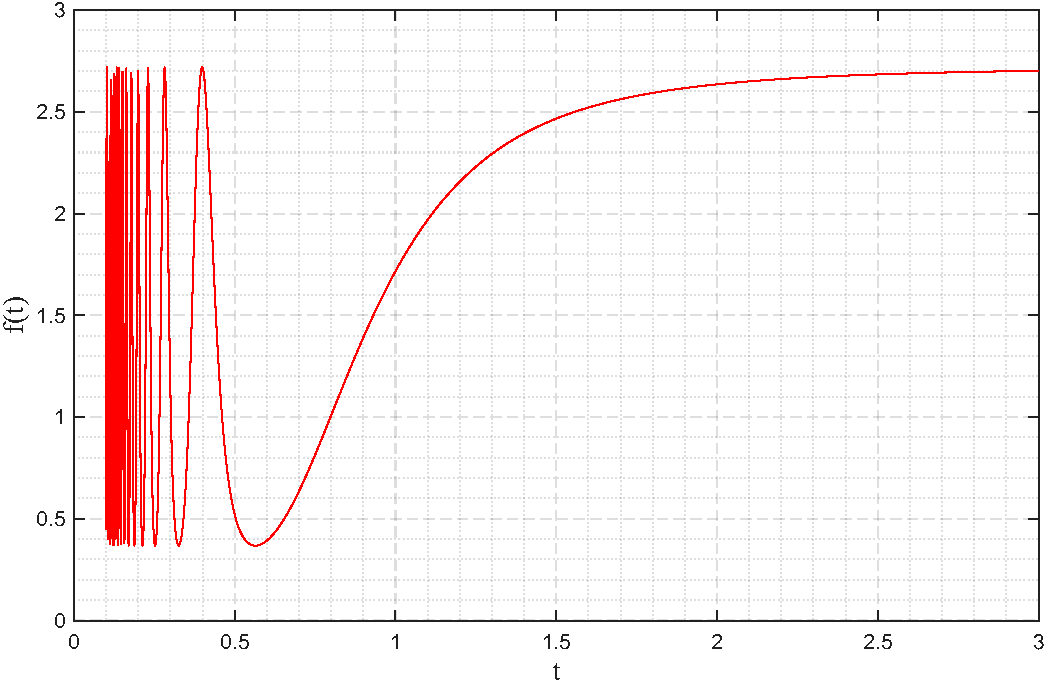
\includegraphics[width=0.8\textwidth]{imagenes/funcion_ft.pdf}
    \caption{Gráfico de $f(t)$}
    \label{fig:1}
\end{figure}

Se observa que integrar es mucho más fácil entre $[0.5, 3]$ pero en $[0.1, 0.5)$ la integración es mucho más difícil debido a las oscilaciones en esa zona, por lo tanto se requiere un paso de integración más chico para considerar los cambios bruscos cercanos al 0.

Claramente la función es no elemental y por lo tanto no se puede encontrar una primitiva. La única forma de evaluar la integral es mediante método numéricos y distintos métodos que se pueden aplicar en MATLAB. En la figura \ref{fig:simpson_trapecio} se observa la función $g(t)$ y los polinomios de interpolación de primer grado (trapecio) e interpolación de segundo grado (simpson). Por lo tanto, podemos aplicar dichos métodos para aproximar la función. La fórmula del trapecio es:

\begin{equation}
    \int_{a}^{b} f(t) \approx \frac{h}{2}\left(f(t_0) + 2\left(\sum_{i = 1}^{n - 1} f(t_i) + \right) f(t_n)\right) 
\end{equation}

La fórmula de Simpson


\begin{equation}
    \int_{a}^{b} f(t)dt \approx \frac{h}{3}\left[f(t_0) + 4\left(\sum_{i = 1, i\  \text{impar}}^{n - 1} f(t_i)\right)  + 2\left(\sum_{i = 2, i \ \text{par}}^{n - 2} f(t_i)\right) + f(t_n) \right] 
\end{equation}

El siguiente código hecho en MATLAB calcula, de forma numérica y con la propia función \texttt{integral} de MATLAB, la integral de \eqref{eq:2} con un paso de $0.05$.

\begin{lstlisting}
clc
close all

h = 0.05; %paso
t = 0.1:h:3;
ft = exp(cos(-1./t.^2));
%{
Las partes mas faciles para integrar esta funcion
es desde 0.5 hacia adelante. Aunque cumple con
las condiciones de integrabilidad (segun las condiciones
de Riemann), numericamente es dificil resolverlo.
Las partes problematicas son las oscilaciones que tiene
al principio
%}

plot(t, ft, 'r')


%Podemos usar el metodo Simpson o del trapecio

function S = trapecio(func, h)
    %{
    func : funcion a encontrar la integral
    h : paso de integracion
    %}
    S = h/2*(func(1) + 2*sum(func(2:end-1)) + func(end));
end


function S = simpson(func, h)
    A = h/3*(func(1) + func(end));
    n = length(func);
    for i = 2:1:n-1
        if mod(i, 2) == 0
            A = A + h/3*4*func(i);
        else
            A = A + h/3*2*func(i);
        end
    end
    S = A;
end


ft_trapecio = trapecio(ft, h);
>>  6.14458158849869

ft_simpson = simpson(ft, h);
>>  6.09083232859325

ft_matlab = integral(@(t) exp(cos(-1./t.^2)), 0.1, 3);
>> 6.03513177870255
\end{lstlisting}

Si ahora hacemos que el paso sea $0.001$ se obtienen resultados muy próximos al valor de $6.035$.

Podemos resolver la integral mediante métodos de ecuaciones diferenciales. Consideremos la expresión de la integral de $f(t)$, es decir:

\begin{equation}
    F(t) = \int f(t)dt
\end{equation}

Por el teorema fundamental del cálculo

\begin{equation}
    \dot{F}(t) = f(t)
\end{equation}

\noindent donde el lado derecho no es más que la expresión \eqref{eq:1}. Tenemos una ecuación diferencial de primer grado y por lo tanto podemos aplicar métodos como Runge-Kutta de cuarto orden. 




\begin{figure}[ht!]
    \centering
    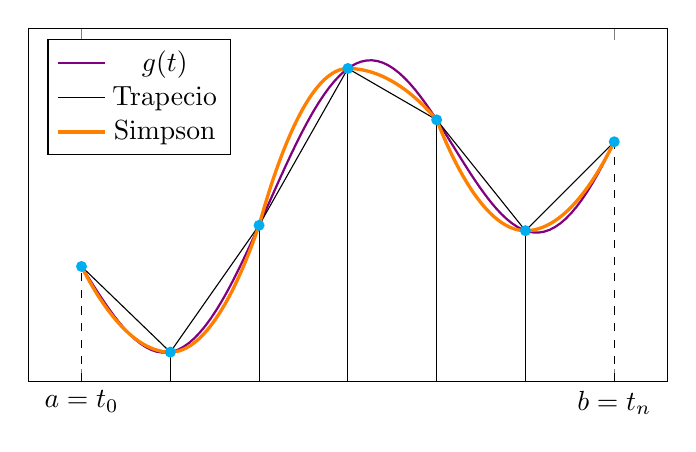
\begin{tikzpicture}
        \begin{axis}[
            trig format = rad,
            xtick = {0, 3},
            ytick = \empty,
            xticklabels = {$a = t_0$, $b = t_n$},
            ymin = 0,
            width = 0.8\textwidth,
            height = 0.5\textwidth,
            legend pos = north west,
        ]

            % Función original
            \addplot[
                domain = 0:3,
                samples = 100,
                violet,
                thick
            ] {2 + x - 2*sin(3*x)};
            \addlegendentry{$g(t)$}

            % Líneas verticales en los extremos
            \draw[dashed] (axis cs:0,0) -- (axis cs:0,2);
            \draw[dashed] (axis cs:3,0) -- (axis cs:3,4.1757);

            % Subintervalos
            \draw (axis cs:0.5,0) -- (axis cs:0.5,0.505);
            \draw (axis cs:1,0)   -- (axis cs:1,2.7177);
            \draw (axis cs:1.5,0) -- (axis cs:1.5,5.455);
            \draw (axis cs:2,0)   -- (axis cs:2,4.5588);
            \draw (axis cs:2.5,0) -- (axis cs:2.5,2.624);

            % Trapecios: unión lineal de los nodos
            \draw[black]
                (axis cs:0,2) --
                (axis cs:0.5,0.505) --
                (axis cs:1,2.7177) --
                (axis cs:1.5,5.455) --
                (axis cs:2,4.5588) --
                (axis cs:2.5,2.624) --
                (axis cs:3,4.1757);
            \addlegendimage{black}
            \addlegendentry{Trapecio}

            % Simpson: interpolación cuadrática por tramos
            \draw[orange, very thick]
                (axis cs:0,2)
                parabola bend (axis cs:0.5,0.505)
                (axis cs:1,2.7177);

            \draw[orange, very thick]
                (axis cs:1,2.7177)
                parabola bend (axis cs:1.5,5.455)
                (axis cs:2,4.5588);

            \draw[orange, very thick]
                (axis cs:2,4.5588)
                parabola bend (axis cs:2.5,2.624)
                (axis cs:3,4.1757);

            \addlegendimage{orange, very thick}
            \addlegendentry{Simpson}

            % Puntos
            \fill[cyan] (axis cs:0,2) circle [radius=0.07cm];
            \fill[cyan] (axis cs:0.5,0.505) circle [radius=0.07cm];
            \fill[cyan] (axis cs:1,2.7177) circle [radius=0.07cm];
            \fill[cyan] (axis cs:1.5,5.455) circle [radius=0.07cm];
            \fill[cyan] (axis cs:2,4.5588) circle [radius=0.07cm];
            \fill[cyan] (axis cs:2.5,2.624) circle [radius=0.07cm];
            \fill[cyan] (axis cs:3,4.1757) circle [radius=0.07cm];

        \end{axis}
    \end{tikzpicture}
    \caption{Aproximación de una integral mediante la regla del trapecio y la regla de Simpson.}
    \label{fig:simpson_trapecio}
\end{figure}


El siguiente código en MATLAB representa la solución a la ecuación diferencial 

\begin{lstlisting}
%Mediante una ecuacion diferencial

function [df] = f21(t, y)
    df = exp(cos(-1./t.^2));
end

opts = odeset('RelTol',1e-7,'AbsTol',1e-4);
%Si agrego el opts mejora la precision
%https://la.mathworks.com/help/matlab/ref/ode45.html?s_tid=ta_help_results
%Primer Metodo
[T1, Y1] = ode45(@f21, [0.1, 3], 0.1, opts);
ft_ode45 = Y1(end) - Y1(1);
>> 6.03679802230507

%Segundo metodo
[T2, Y2] = ode15s(@f21, [0.1, 3], 0.1, opts);
ft_ode15 = Y2(end) - Y2(1);
>> 6.03098868384105

%Tercer metodo
[T3, Y3] = ode23s(@f21, [0.1, 3], 0.1, opts);
ft_ode23 = Y3(end) - Y3(1);
>> 6.03404436431533 
\end{lstlisting}


La función \texttt{ode45}, \texttt{ode15s}, \texttt{ode23s} reciben, principalmente, 3 argumentos: el lado derecho a resolver, el \texttt{tspan} o dominio de integración y las condiciones iniciales. El cuarto argumento sirve para agregar opciones de tolerancias a errores absolutos y relativos. Aunque las 3 funciones sirven para integrar ecuaciones diferenciales se diferencian en:

\begin{itemize}
    \item \texttt{ode45} : Utiliza Runge-Kutta de cuarto orden. Tiene propósitos generales pero no funciona muy bien para ecuaciones diferenciales rígidas (cambios muy bruscos).
    \item \texttt{ode23s} : Utiliza Runge-Kutta de segundo orden. Aunque sea menos preciso que RK4(5) sirve para resolver ecuaciones diferenciales rígidas.
    \item \texttt{ode15s} : está basado en fórmulas de diferenciación numérica.
\end{itemize}


Se observa que cambiando la tolerancia relativa ésta misma cambia los valores de los resultados. Sí se puede confiar en los resultados dados por los métodos numéricos, porque a pesar de que son aproximaciones los resultados son certeros debido a que también existe un resultado de los errores para cada iteración. Si sabemos cómo controlar estos errores (mejorando el método, cambiando las tolerancias, reduciendo el paso, etcétera) entonces podemos asegurar los resultados. Cabe aclarar que juega mucho el conocimiento sobre el tema y saber interpretar los resultados, porque pese a que MATLAB pueda resolver ecuaciones diferenciales, los resultados tienen que tener sentido y eso dependerá del análisis y fenómeno el cual se trata.  


Por último, definamos variables simbólicas para integrar en MATLAB. Veamos lo siguiente:

\begin{lstlisting}
syms x z a
f = 3*a+x;
int_f = int(f); %Integra con respecto a x si no pongo nada
>> (x*(6*a + x))/2
\end{lstlisting}

Integró con respecto a la variable \texttt{x}. Ahora, si especificamos que queremos integrar con respecto a la variable \texttt{a}, entonces


\begin{lstlisting}
syms x z a
f = 3*a+x;
int_f = int(f, a); 
>> (a*(3*a + 2*x))/2
\end{lstlisting}


Veamos ahora el ejemplo de integrar $g(x, z) = x / (1+z^2)$ con respecto a la variable $x$ y $z$.


\begin{lstlisting}
g = x / (1+z^2);
int_g_x = int(g, x);
>> x^2/(2*(z^2 + 1))

int_g_z = int(g, z);
>> x*atan(z)
\end{lstlisting}


\noindent Donde \texttt{atan} representa el arcotangente.

Por último, veamos el ejemplo de integrar la siguiente función

\begin{equation}
    f(x) = e^{x^2}
\end{equation}


\noindent con respecto a $x$. Si hacemos esto en MATLAB obtenemos lo siguiente:

\begin{lstlisting}
h = exp(x^2);
int_h = int(h);
>> (pi^(1/2)*erfi(x))/2
\end{lstlisting}


Para saber qué función es erfi, nos basamos en el libro \textit{Table of Integrals, Series, and Products} de I.S. Gradshteyn y I.M. Ryzhik (página 157, sección 2.33, fórmula 2):

\begin{equation}
    \int e^{ax^2}dx = \frac{1}{2}\sqrt{\frac{\pi}{a}} \text{erfi}\ (\sqrt{a}x)
\end{equation}


\noindent donde para nuestro caso $a = 1$ y erfi = erf($ix$)/$i$, donde 


\begin{equation}
    \text{erf}(ix) = \frac{2}{\sqrt{\pi}}\int_{0}^{ix} e^{-t^2}dt 
\end{equation}

\noindent es la función error. 



